
\section{Average number of generations until equilibrium}\label{sec:aantgen}
There are numerous parameters that may affect the average number of generations until  equilibrium is reached. 
We chose to focus on the effect of the Happiness Rule(HR) on the average number of generations. 
For each HR ranging from 0 to 1 with increment 0.01, we ran 500 simulations and calculated the average, maximal and minimal generations it took to reach equilibrium. 
The results are shown in figure \ref{fig:avegen}.\\

From figure \ref{fig:avegen}, we conclude that the average number of generations (blue graph) is increasing with the Happiness Rule, which is to be expected since a higher HR implies a higher need for neighbours of the same type, and thus a lower probability that a selected individual is happy, making it more likely that he/she will move. 
We also note that starting at a HR of aproximately 0.7, the average number of generations appears to be nearly constant. 
This can be explained noting that the required number of neighbours will practically be the same. 
For example, if the HR were 0.8, a person with 3, 5 or 8 neighbours would require respectively 3, 5 or at least 7 of the same type. 
This requirement hardly changes if a HR of 0.9 is applied. 
The same argument explains why the average number of generations is constant at very low HR or if we raise the HR with a sufficiently small amount like $0.01$.

\begin{figure}[h!]
    \centering
    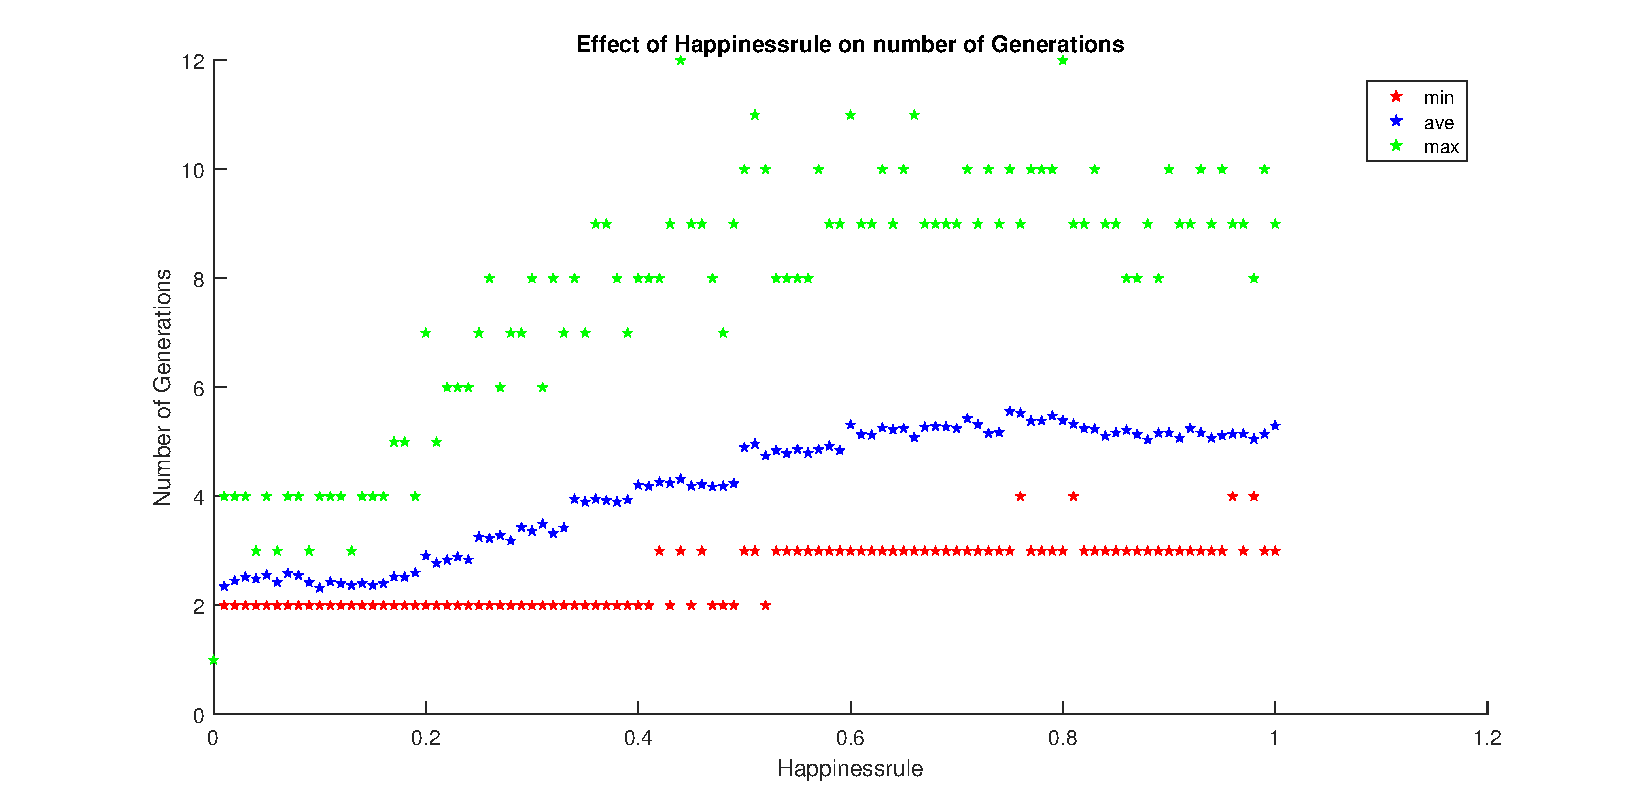
\includegraphics[width=0.9\textwidth]{happinessregel_aantgen_2.pdf}
    \caption{Effect of the happiness rule on the number of generations until reaching equilibrium. 
    The green graph represents the maximal number of generations, the blue graph the average number of generations and the red graph displays the minimal number of generations}
    \label{fig:avegen}
\end{figure}
<<<<<<< HEAD
\\
It is also interesting to investigate how the random variables $Y_j$, which we denote as the number of generations it takes to reach the equilibrium under HR $j$, is distributed, and how their distributions are affected by the HR. For this purpose, we ran 10000 simulations for Happiness Rules of 1/4,1/3,1/2 and 1 and plotted several histograms (figure\ref{fig:histogram}). We chose bin size 1 for each histogram given that $Y_j$ is a random variable that only takes integer values. Therefore, a histogram of a bin size such as 0.5 will not give any additional information and their would be lots of loss of information if bin size 2 is chosen(since we don't have many different generations). 
\\
=======

As is one of the research questions, it is also interesting to investigate how the random variables $Y_j$, which we denote as the number of generations it takes to reach the equilibrium under HR $j$, is distributed, and how their distributions are effected by the HR. 
For this purpose, we ran 10000 simulations for with Happiness Rules of 1/4,1/3,1/2 and 1 and plotted several histograms (figure\ref{fig:histogram}). 
We chose bin size 1 for each histogram given that $Y_j$ is a random variable that only takes integer values. 
Thus a histogram of a bin of for example $0.5$ will not give any additional information and their would be a severe loss of information if bin size $2$ is chosen. 
>>>>>>> c7720a2dd5b3d68d165db322469323054a50e3ed

\begin{figure}[H]
    \centering
    \begin{subfigure}{0.45\textwidth}
        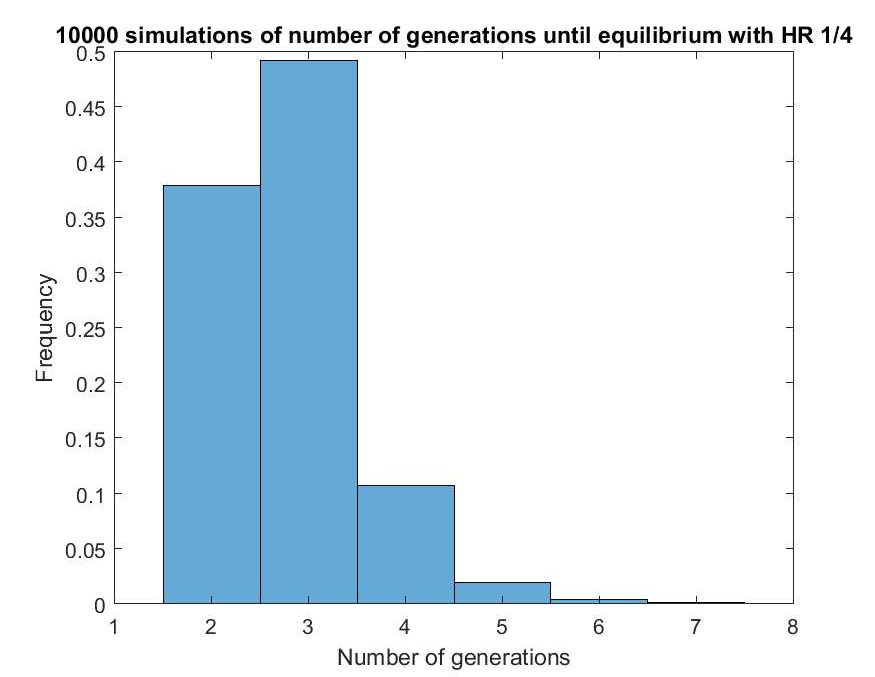
\includegraphics[width=\textwidth]{GenormHistogramAantalgen4.pdf}
        \caption{10000 simulations of number of generations until equilibrium with HR 1/4}
        \label{hist hap 1/4}
    \end{subfigure}
	~
    \begin{subfigure}{0.45\textwidth}
        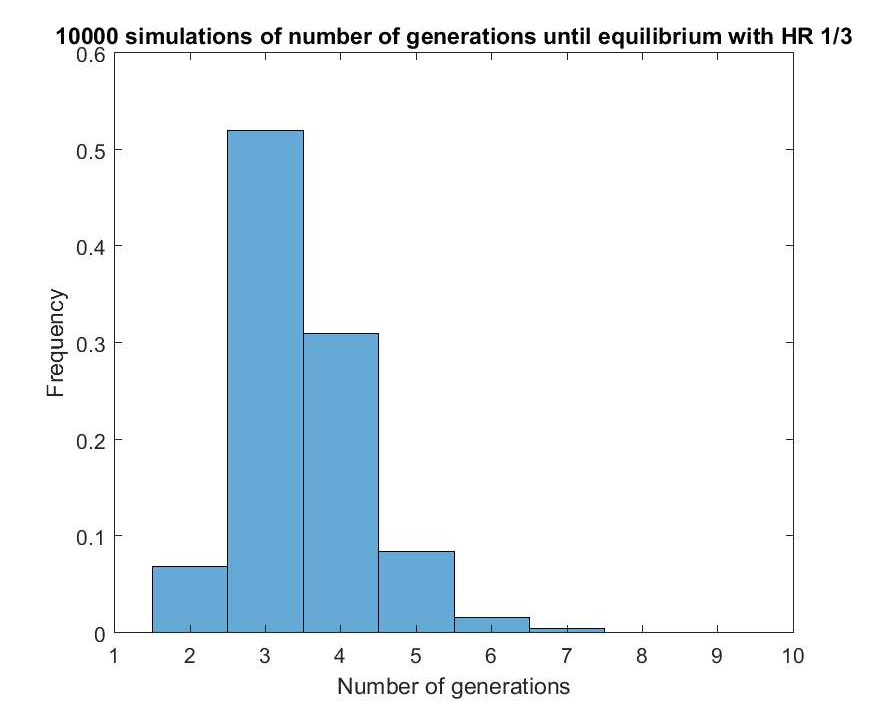
\includegraphics[width=\textwidth]{GenormHistogramAantalgen.pdf}
        \caption{10000 simulations of number of generations until equilibrium with HR 1/3}
        \label{hist hap 1/3}
    \end{subfigure}
	~
    \begin{subfigure}{0.45\textwidth}
        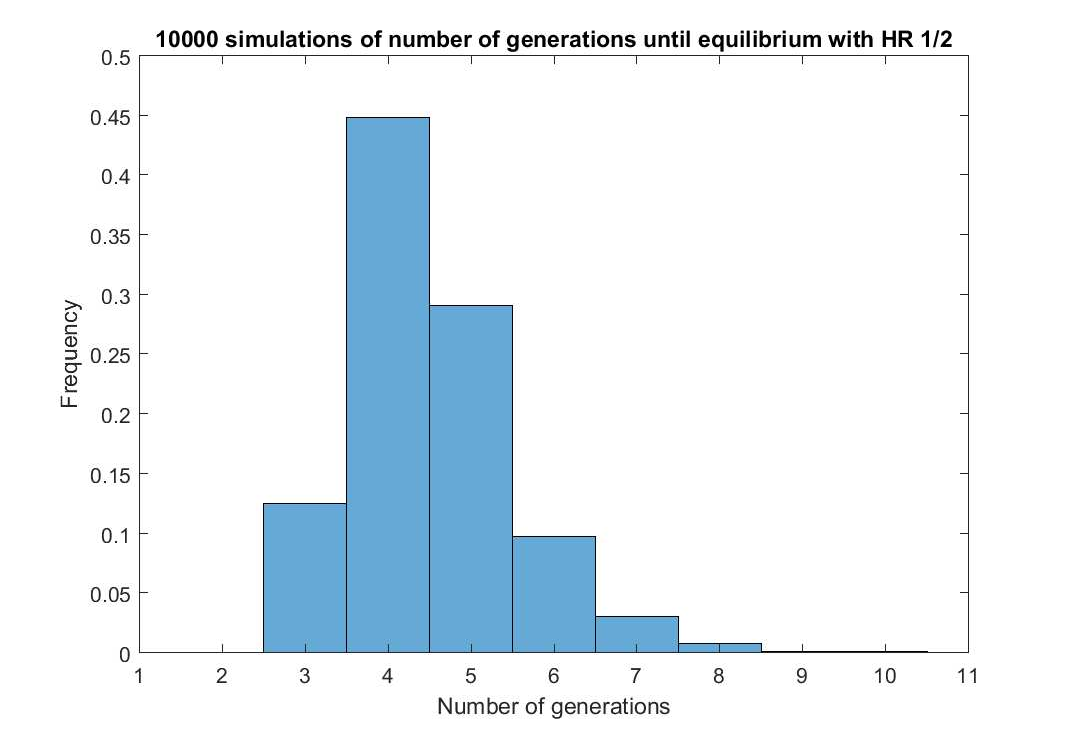
\includegraphics[width=\textwidth]{GenormHistogramAantalgen2.pdf}
        \caption{10000 simulations of number of generations until equilibrium with HR 1/2}
        \label{hist hap 1/2}
    \end{subfigure}
    ~
    \begin{subfigure}{0.45\textwidth}
        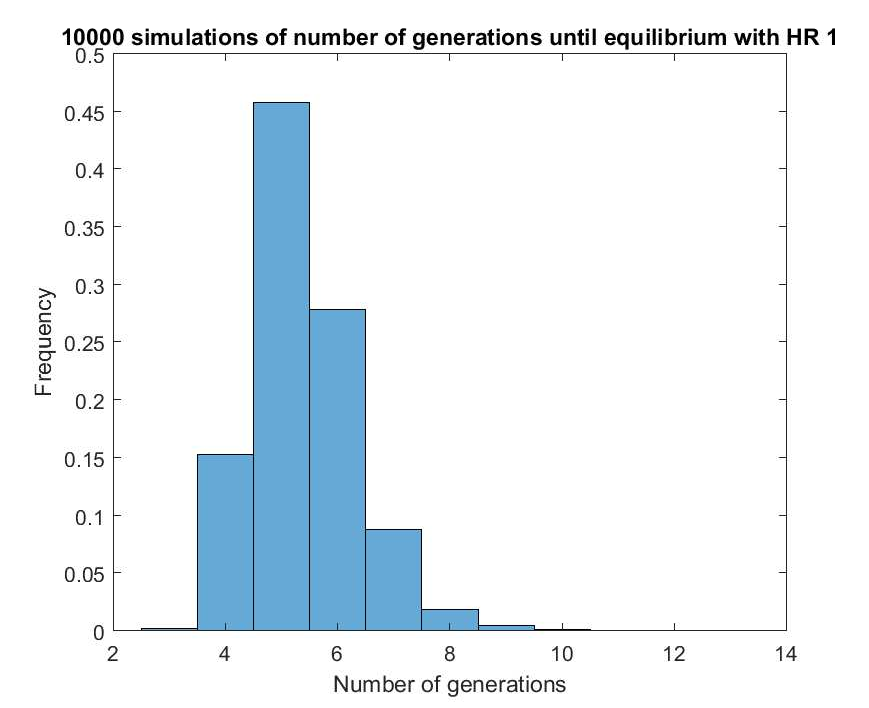
\includegraphics[width=\textwidth]{GenormHistogramAantalgen1.pdf}
        \caption{10000 simulations of number of generations until equilibrium with HR 1}
        \label{hist hap 1}
    \end{subfigure}
    \caption{The probability distribution of $Y$ (the number of generations until reaching the equilibrium) is approximated with a histogram of bin size 1. 
    For each HR ($1/4$, $1/3$, $1/2$ and $1$), $10000$ simulations were ran.}
    \label{fig:histogram}
\end{figure}

<<<<<<< HEAD
Looking at the histograms, all $Y_j$'s ($j\in \{1/2,1/3,1/4,1\}$) might come from the same distribution, but with different parameters, since their sample means are obviously different.\\
\\
For simplicity, we chose to only investigate the distribution of $Y_{1/3}$, since other $Y_j$'s might follow the same family distribution as suggested by the histrograms. We suspected that $Y_{1/3}$ might be Poisson distributed. So with this assumption, we first used the 'fitdist'-function of Matlab to calculate the maximal likelihood estimater $\hat{\lambda}$ for the real Poisson parameter $\lambda$. Then, we performed the chi-sqaured test using the chi2gof function in Matlab, with null-hypothesis $H_0:F_{1/3}=F_{P,\hat{\lambda}}$, for which $F$ is the unknown cumulative distribution function(CDF) from the data and $F_{P,\hat{\lambda}}$, the CDF from Poisson$(\hat{\lambda})$. The alternative hypothesis is $F_{1/3}\neq F_{P,\hat{\lambda}}$. Furthermore, we chose 8 bins for the chi-sqaured test(otherwise the test is not accurate due to low expected counts in some bins). The test has rejected the null-hypothesis and the test was of significance level $\alpha=0.05$. \\   
\\
With the same method, we've also tested whether $Y_{1/3}$ is binomial or negative binomial distributed. But again, they have been rejected by the chi-sqaured test. So we can only conclude that $Y_{1/3}$ is not Poisson, binomial and negative binomial distributed.\\
We've also performed this statistical analysis on other $Y_j$'s(for instasnce $Y_1$), and we've obtained the same result as for $Y_{1/3}$.\\
\\
In order to make a better comparison of the distribution between $Y_{1/3},Y_{1/4},Y_{1/2}$ and $Y_1$, we made some QQ-plots, which is shown in figure \ref{fig:QQ-plot}.\\ 
=======
Looking at the histograms in figure \ref{fig:histogram}, all $Y_j$'s ($j\in \{1/2,1/3,1/4,1\}$) might come from the same distribution, but with different parameters, since their sample means are obviously different.\\
In an attempt to find a good (confidence level $95\%$) fit for the distribution of $Y_{1/3}$, we've used the chi-squared goodness of fit test(chi2gof) to see whether $Y_{1/3}$ is Poisson distributed. 
We first used the 'fitdist'-function of Matlab to calculate the maximal likelihood estimater for $\hat{\lambda}$ and then performed the chi-sqaured test. 
The test has rejected the null-hypothesis $H_0:Y_{1/3}\sim\text{Poisson}(\hat{\lambda})$ with significance level $\alpha=0.05$.\\   

With the same method, we've also tested whether $Y_{1/3}$ is binomial or negative binomial distributed. 
But again, they have been rejected by the chi-squared test. 
So we can only conclude that $Y_{1/3}$ is not Poisson, binomial and negative binomial distributed.\\

In order to make a better comparison of the distribution between $Y_{1/3},Y_{1/4},Y_{1/2}$ and $Y_1$, we made some QQ-plots, which is shown in figure \ref{fig:QQ-plot}.
 
>>>>>>> c7720a2dd5b3d68d165db322469323054a50e3ed
\begin{figure}[H]
    \centering
    \begin{subfigure}{0.8\textwidth}
    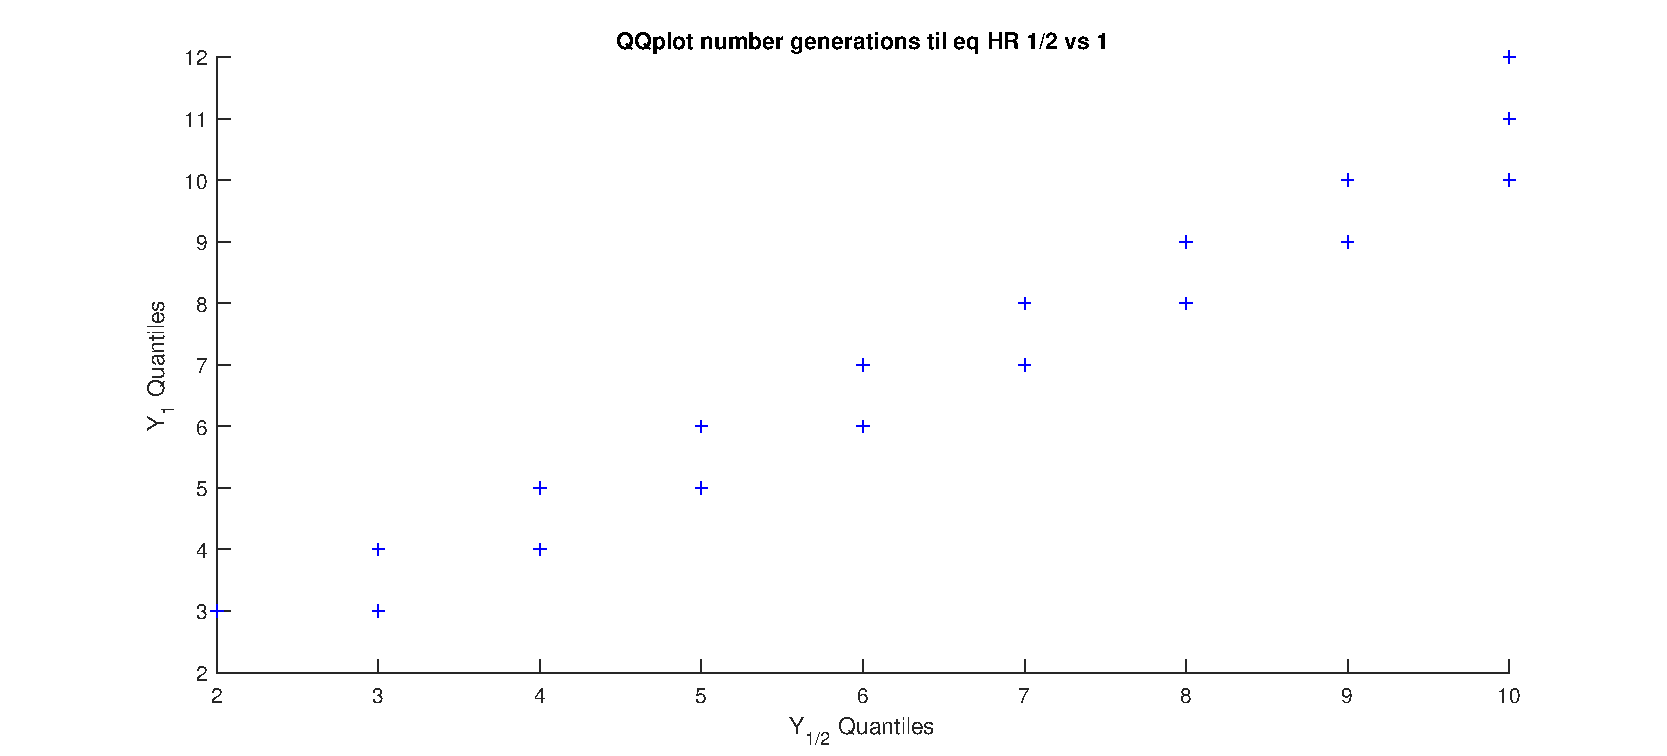
\includegraphics[width=\textwidth]{QQplotATGEN3.pdf}
    \caption{QQ-plot of $Y_{1}$ vs $Y_{1/2}$}
        \label{fig:QQplotATGEN3}
    \end{subfigure}
    
    \begin{subfigure}{0.8\textwidth}
    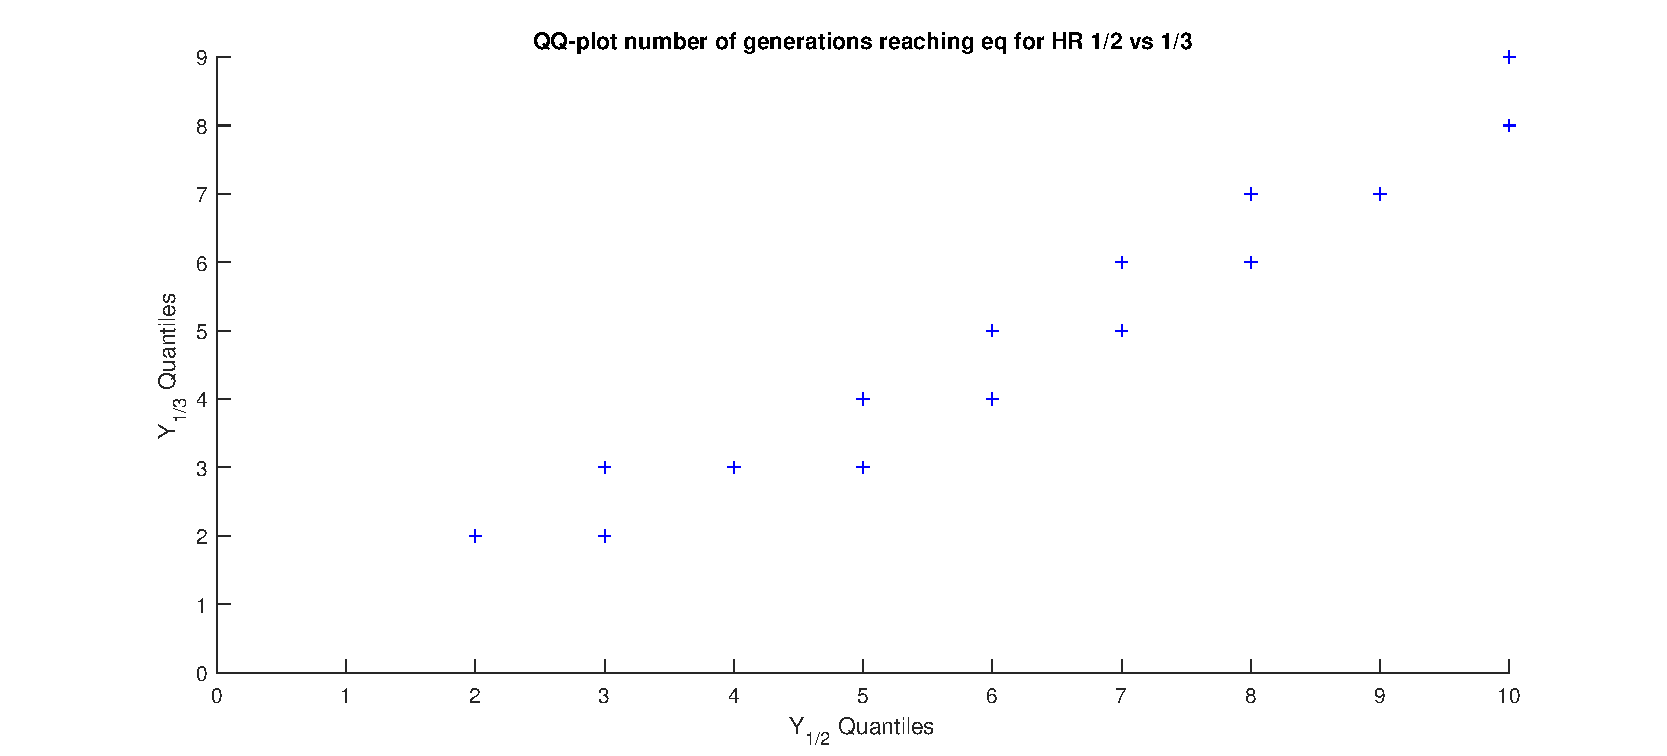
\includegraphics[width=\textwidth]{QQplotATGEN1.pdf}
    \caption{QQ-plot of $Y_{1/3}$ vs $Y_{1/2}$}
        \label{fig:QQplotATGEN1}
    \end{subfigure}
    \begin{subfigure}{0.8\textwidth}
    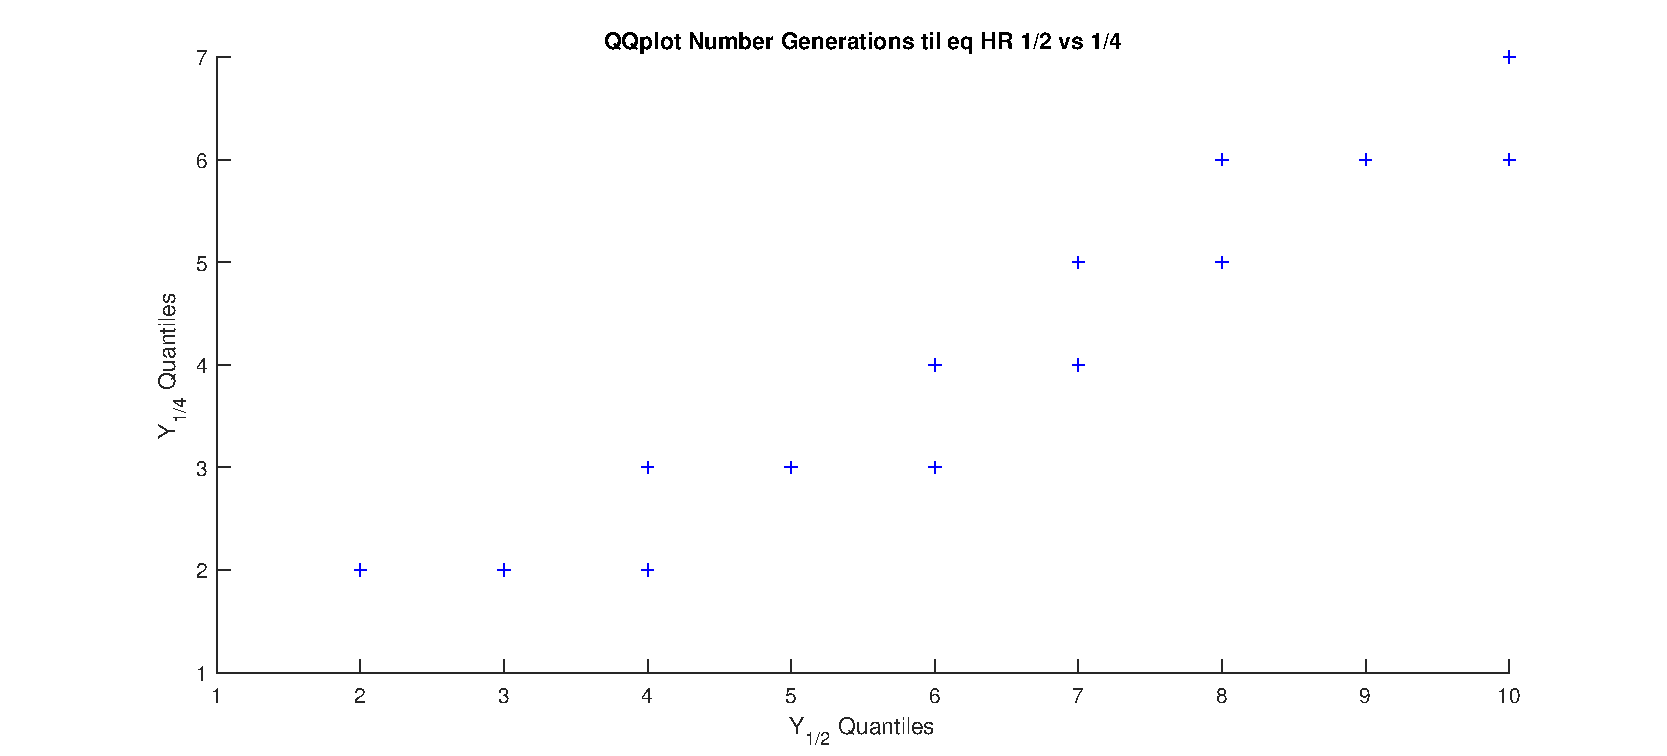
\includegraphics[width=\textwidth]{QQplotATGEN2.pdf}
    \caption{QQ-plot of $Y_{1/4}$ vs $Y_{1/2}$}
        \label{fig:QQplotATGEN2}
    \end{subfigure}
    \caption{QQ-plot of $Y_{1}$ vs $Y_{1/2}$, $Y_{1/3}$ vs $Y_{1/2}$ and $Y_{1/4}$ vs $Y_{1/2}$}
    \label{fig:QQ-plot}
\end{figure}
<<<<<<< HEAD
As expected, the QQ-plots have a stairwise pattern. This is because our data came from a discrete random variable. We see that the plots appears linear, especially the plot of $Y_{1}$ vs $Y_{1/2}$. The plot indicates that these 4 $Y_j$'s might belong to the location-scale family of some distribution.\\
\\
With the two-sample kolomogorov-smirnov test (kstest2) of significance level $\alpha=0.05$ in Matlab, which has null-hypothesis $H_0:F(X)=G(Y)$ for $F,G$ the CDF of $X$ and $Y$, and $H_1: F(X)\neq G(Y)$, it can be concluded that these $Y_j$'s don't come from the same distribution with the same parameters. Unfortunately, we weren't able to find a test that tests whether these $Y_j$'s comes from the same family distribution (i.e. same distribution but different parameter values).\\
\\
%A fact worth noting, is that both the mean and the variance increase with the happiness rule. In line with the following section, the mean remains fairly low, while the number of generations tend to be fairly spread.\\
%\textbf{Partial explanation.} While not immediately intuitive, the relatively small mean cannot be immediately explained. We do have an explanation for the relatively high frequency of the large number of generations however: If, after a few generations, equilibrium is not reached, the chance to move to a proper location decreases. Further details of this are provided in the following section. Thus, reaching equilibrium costs a fairly great amount of time.
=======

As expected, the QQ-plots have a stairwise pattern. 
This is because our data came from a discrete random variable. 
We see that the plots appears linear, especially the plot of $Y_{1}$ vs $Y_{1/2}$. 
The plot indicates that these 4 $Y_j$'s might belong to the location-scale family of some distribution.\\

With the two-sample kolomogorov-smirnov test (kstest2) of significance level $\alpha=0.05$ in Matlab, which has null-hypothesis $H_0:F(X)=G(Y)$ for $F,G$ the CDF of $X$ and $Y$, it can be concluded that these $Y_j$'s don't come from the same distribution with the same parameters. 
Unfortunately, we weren't able to find a test that tests whether these $Y_j$'s comes from the same family distribution (i.e. same distribution but different parameter values).\\

A fact worth noting, is that both the mean and the variance increase with the happiness rule. In line with the following section, the mean remains fairly low, while the number of generations tend to be fairly spread.\\

\textbf{Partial explanation.} \\
While not immediately intuitive, the relatively small mean cannot be immediately explained. We do have an explanation for the relatively high frequency of the large number of generations however: 
If equilibrium is not reached after a few generations, the chance to move to a proper location decreases. 
Further details of this are provided in the following section. 
Thus, reaching equilibrium costs a fairly great amount of time.
>>>>>>> c7720a2dd5b3d68d165db322469323054a50e3ed

